\chapter{Introduzione}

\section{Obiettivi}
L’obiettivo è lo studio della blockchain di Litecoin per effettuare una comparazione con Bitcoin. A tal fine ho svolto delle analisi riguardanti prevalentemente il lato tecnologico di essa, lo sviluppo, le applicazioni, ma anche il lato economico, tramite dati esterni, come fees, exchange rates e la loro evoluzione nel tempo.
\section{Contributi}
Per l’analisi della blockchain Litecoin ho esteso il tool BlockAPI, implementando le strutture dati e le queries necessarie a tal fine. La parte tecnica dell’estensione del tool verrà discussa nel capitolo 2.
\section{Struttura della tesi}
La tesi presenta un background tecnico iniziale necessario a capire Bitcoin e valido per tutte le criptovalute da esso derivate e mostra le caratteristiche principali per cui Litecoin differisce da Bitcoin. Segue un’introduzione delle tecnologie utilizzate e del mio contributo al tool che è stato utilizzato per l’analisi. Infine le analisi, per ciascuna delle quali viene illustrato un contesto per comprenderla, lo svolgimento di essa, il codice e le queries ed i risultati numerici e loro eventuali rappresentazioni grafiche.

\section{Background}
\subsection{Bitcoin}
Bitcoin è una criptovaluta nata nel 2009 ad opera di Satoshi Nakamoto, la cui vera identità è ancora ignota. Open source, orientata all’anonimato, decentralizzata e peer to peer, non possiede alcun server “centrale” o organismo di controllo. È una risorsa totalmente virtuale che non prevede un’unità fisica associata: i Bitcoin sono “coniati” tramite un processo, il cosiddetto mining, che comporta una competizione nel cercare le soluzioni di un problema computazionale estremamente oneroso da risolvere ma la cui soluzione sia semplicissima da verificare, detto Proof of Work.
Chiunque può minare tramite la potenza di calcolo di cui dispone, ma la difficoltà del puzzle crittografico viene ricalcolata ogni 2016 blocchi -approssimativamente 2 settimane- in base alla potenza di calcolo del network affinché in media un blocco di transazioni sul network venga generato e validato ogni 10 minuti. Dunque ogni 10 minuti circa un nuovo blocco viene confermato e aggiunto alla blockchain e questo lavoro viene ricompensato con una quantità prestabilita di Bitcoin nuovi di zecca. 
La ricompensa per il miner si dimezza circa ogni 4 anni perché, dal momento che il protocollo Bitcoin permette l’esistenza di massimo 21 milioni di unità monetarie, la ricompensa deve essere sufficientemente elevata da incentivare il lavoro del miner ma non così tanto da deprezzare la valuta mettendo in circolazione prematuramente un numero eccessivo di Bitcoin. Attualmente la ricompensa ammonta a 12.5 BTC e nel 2020 subirà un nuovo dimezzamento.\cite{blockonomi}
Le informazioni e lo storico di tutte le transazioni sulla rete sono immutabili e distribuiti sui nodi che la costituiscono. La struttura dati atta a garantire ciò è la Blockchain e tramite essa Bitcoin decentralizza e distribuisce sulla rete le funzioni di emissione di valuta (mining) e di compensazione (halving) eliminando la necessità di una banca centrale.



\subsubsection{Background tecnico}
Per capire Bitcoin è utile chiarire cosa sia effettivamente una transazione in Bitcoin e in cosa differisca da una “ordinaria”, ad esempio con carta di credito. Il concetto di transazione bancaria che conosciamo prevede una privacy ferrea e l’utilizzo della crittografia al fine di non far intercettare dati sensibili ai malintenzionati, mentre in questo caso la transazione è pubblicamente disponibile per intero in un registro pubblico immutabile e non contiene dati personali. Bitcoin ha praticamente trasformato i soldi in una struttura dati e fatto in modo che sia quasi impossibile per chiunque creare una transazione illeggittima, ma che allo stesso tempo sia facilissimo verificarne la validità. Una transazione è infatti una struttura dati che codifica e trasferisce un valore da una fonte di fondi, detta input, ad una destinazione, detta output. La tabella 1.1 riporta la struttura dell'header di una transazione.

\begin{table}[ht]
	\centering
	\resizebox{\textwidth}{!}{
\begin{tabular}{|c|c|c|}
\hline
\textbf{	 
	Dimensione }&\textbf{ Campo }&\textbf{ Descrizione }\\ \hline
 
	 
4 Bytes	& Versione & Specifica quali regole segue la transazione \\ \hline
 
	 
1-9 Bytes (VarInt)	& Input Counter &  Quanti input sono inclusi\\ \hline
 
Variable	& Inputs &  Uno o più input di transazione\\ \hline
 	 
1-9 Bytes (VarInt)	& Output Counter &  Quanti output sono inclusi \\ \hline
 	 
Variable	& Outputs &  Uno o più input di transazione\\ \hline
 	 
4 Bytes	& Locktime & Un Unix timestamp o numero del blocco \\ \hline
\end{tabular}}
\caption{Struttura dell'header di una transazione Bitcoin \cite{masteringbitcoin}}
\end{table}


I componenti di una transazione sono i cosiddetti UTXO, o input di transazione non spesi, la cui aggregazione dà il “saldo” dell’utente -in Bitcoin non esiste un vero e proprio concetto di saldo- e il resto di un UTXO più grande del valore desiderato viene restituito, in modo analogo, come UTXO più piccolo (che assume il valore del resto). 
Ogni transazione Bitcoin contiene almeno un input e output, ad eccezione delle transazioni coinbase che contengono un solo output del valore della ricompensa per il miner, già precedentemente accennata. Tutti gli outputs ad eccezione dei cosiddetti OP\_RETURN producono a loro volta bitcoin spendibili e sono composti da un importo in bitcoin e un “locking script” che ha la funzione di verifica: solo chi soddisfa le condizioni poste dallo script può riscattare l’output. La transazione viene firmata tramite la chiave privata del proprietario e può essere sbloccata solo dall’indirizzo del destinatario legittimo.
Chiunque voglia ricevere un pagamento, o effettuarne uno, necessita di una copia pubKey:privateKey.Ogni partecipante al network crea tramite il client una privateKey di 256 bit che occorrerà per firmare la transazione.
Da questa chiave si genera successivamente la pubKey di 512 bit, tramite l’algoritmo ECDSA su curva ellittica secp256k1.
Tale chiave verrà usata per la verifica dell'autenticità della firma digitale del mittente.  
Per sicurezza e praticità si esegue un doppio hash: per prima cosa si calcola SHA-256(PubKey), e successivamente si esegue RIPEMD-160(SHA-256(PubKey)); per ottenere l'indirizzo si utilizza una ulteriore codifica in Base58Check per ottenere un indirizzo in formato standard.


\begin{figure}[h!]
\centering
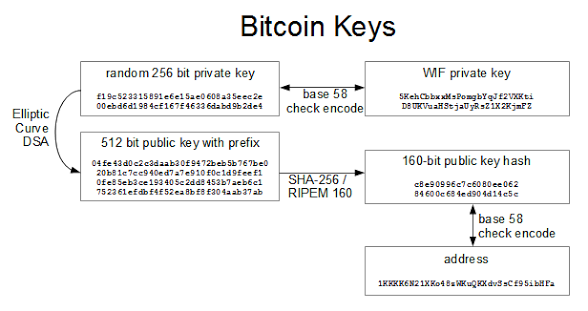
\includegraphics[width=0.9\linewidth]{EcdsaToAddress-bstavroulakis}
\caption{Processo di codifica di un indirizzo bitcoin (bstavroulakis.com)}
\label{fig:ecdsatoaddress-bstavroulakis}
\end{figure}


Ogni transazione validata dal network viene inserita in un blocco di transazioni che è accodato alla blockchain.
La blockchain è un registro pubblico e distribuito che tiene traccia di tutte le transazioni che sono state effettuate fin dal primo blocco. È immutabile e ciascun nodo ne contiene una copia: ai fini di questa tesi non è necessario dettagliare il sistema di consenso (la Proof of Work precedentemente citata) ma è fondamentale ricordare che l’intero sistema si basa su di esso e, soprattutto, che la versione “ufficiale” della blockchain è quella su cui il maggior numero di nodi sono d’accordo. Ciò che rende estremamente sicura la blockchain è proprio l’utilizzo della curva ellittica in associazione alle funzioni di hashing precedentemente citate, SHA-256 e RIPEMD-160, che processano l’input X producendo in output una stringa di lunghezza fissa H(X) da cui non poter ricavare l’input originario X. Inoltre, minime variazioni di X possono portare variazioni enormi in H(X) ed essa non deve contenere una pre-immagine di X.

\begin{figure}[h!]
\centering
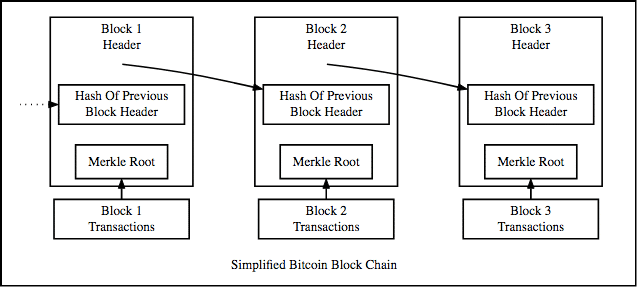
\includegraphics[width=1.0\linewidth]{SimplifiedBlockchainBlockGeeks}
\caption{Struttura semplificata di una blockchain}
\label{fig:simplifiedblockchainblockgeeks}
\footnote{Fonte blockgeeks.com}
\end{figure}


La blockchain è una lista concatenata che contiene dati e un hash pointer che punta al blocco precedente. Un hash pointer differisce da un normale puntatore perché invece di limitarsi a contenere l’indirizzo del blocco precedente contiene anche l’hash dei dati del blocco che punta. Nel caso di Bitcoin, inoltre, la funzione di hashing viene applicata doppiamente nell’header in due casi.\\

% \usepackage[table]{xcolor} is necessary !
\begin{table}[ht]
	\centering
	\resizebox{\textwidth}{!}{
\begin{tabular}{|c|c|c|c|}
	\hline
	\textbf{Bytes} &       \textbf{Name}        & \textbf{Data Type} &                     \textbf{Description}                     \\ \hline
	      4        &          version           &      int32\_t      &   Indica il set di regole utilizzato per la validazione del blocco.   \\ \hline
	      32       & previous block header hash &      char[32]      &            Hash dell'header del blocco precedente           \\ \hline
	      32       &      merkle root hash      &      char[32]      &                Hash in internal byte order derivato dagli hash delle transazioni.                \\ \hline
	      4        &            time            &     uint32\_t      & Unix timestamp del momento in cui il miner ha iniziato l'hashing dell'header \\ \hline
	      4        &           nBits            &     uint32\_t      &  
	      Codifica del valore target per la validazione dell'hash\\ \hline
	      4        &           nonce            &     uint32\_t      & 
	      Numero arbitrario, modificabile dal miner per rispettare nBits \\ \hline
\end{tabular}}
\caption{Struttura dell'header di un blocco Bitcoin (documentazione ufficiale bitcoin.org)}
\end{table}


Nella tabella 1.2 possiamo osservare la struttura degli 80 Bytes dell’header di ciascun blocco. Tenendo presente quanto affermato in precedenza sulle funzioni di hashing risulta chiara la virtuale impossibilità di riuscire ad effettuare qualsivoglia modifica senza che questa abbia un impatto sull’intera blockchain.

\begin{figure}
	\centering
	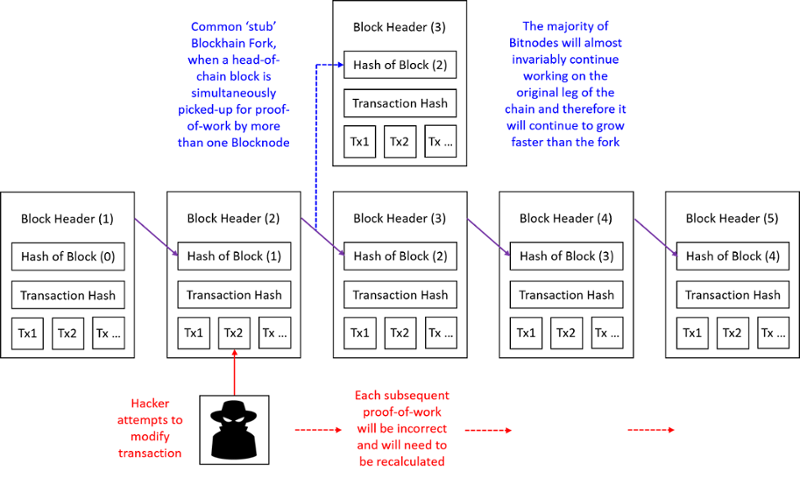
\includegraphics[width=1.0\linewidth]{images/blockchain-diagram}
	\caption{Impatto della modifica di una transazione sulla blockchain: ogni proof-of-work successiva risulterà scorretta e necessiterà il ricalcolo, mentre la maggioranza dei nodi continuerà a lavorare sui dati della blockchain corretta.}
	\label{fig:blockchain-diagram}
\end{figure}


È questo a garantire l’inalterabilità del contenuto della blockchain: oltre alla difficoltà data dalla potenza computazionale richiesta per rendere almeno fattibile l’attacco, il costo lo rende nella quasi totalità dei casi insostenibile o non profittevole.
A titolo d’esempio, riporto la stima di quanto costerebbe sferrare un attacco alle principali blockchain allo stato attuale

\begin{figure}[h]
\centering
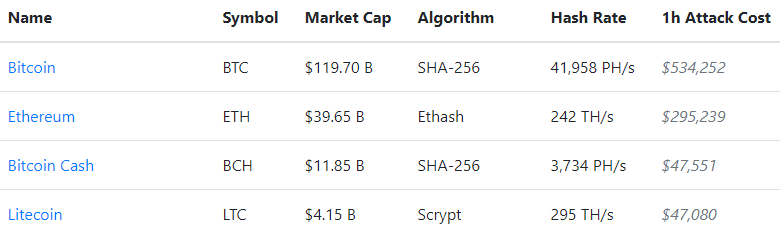
\includegraphics[width=1.0\linewidth]{51cost2therevenge}	
\caption{Costo stimato di un attacco alle principali valute (crypto51.app, agosto 2018)}
\label{fig:51cost2therevenge}
\end{figure}



In breve: la blockchain è un registro pubblico immutabile contenente una serie di blocchi di transazioni validate, ognuna delle quali consiste in un trasferimento di fondi da uno o più input non spesi ad uno o più output, e tutto ciò avviene in modo decentralizzato ed è reso sicuro tramite le curve ellittiche e funzioni di hashing che garantiscono che solo i legittimi proprietari possano usufruire dei fondi.



\subparagraph{Forks e Altcoins}

L’esistenza stessa di una blockchain dipende dall’aderenza alle regole dell’intero network. Blocchi che non rispettano le regole non possono essere validati.
Bitcoin, essendo open source, viene mantenuto e valutato da comunità di sviluppatori che reagiscono ai problemi che emergono nel network tramite dei BIP (Bitcoin Improvement Proposal) che formalmente sono uno standard di proposta di miglioramento. Questi possono riguardare il protocollo o le regole. Una soft fork consiste infatti in un cambiamento di protocollo o di regole in modo retrocompatibile: il software continuerà a riconoscere i blocchi precedenti e i vecchi nodi non aggiornati saranno in grado di validare nuovi blocchi. Detta consensus fork, per la sua attuazione è sufficiente che la maggioranza dei miner sia d’accordo. Talvolta si hanno, tuttavia, notizie di attacchi hacker verso i nodi non aderenti (es: DDoS) per forzarne indirettamente l’adesione. Un esempio di soft fork è l’implementazione di SegWit, oggetto di un’analisi al capitolo 4.
Qualora non fosse presente il consenso necessario tra i miners e la nuova versione del software non fosse retrocompatibile si verificherebbe un hard fork: quando ciò si verifica la blockchain subisce una separazione definitiva e il possessore di criptovaluta la possiede ora duplicata sulla blockchain forked.
Un hard fork piuttosto noto di Bitcoin è Bitcoin Cash: differisce dal protocollo originale per la dimensione del blocco, che da 1 passa ad 8 MB. Chi possedeva X bitcoin (BTC) al momento del forking ha potuto ottenere gratuitamente X bitcoincash (BCH).
Infine ci sono le cosiddette altcoins: forks del codice sorgente di Bitcoin, blockchain totalmente separata, differenze di protocollo scarsamente compatibili. Litecoin è definibile a tutti gli effetti una altcoin ed è stata a sua volta oggetto di codebase forks.


\begin{figure}
	\centering
	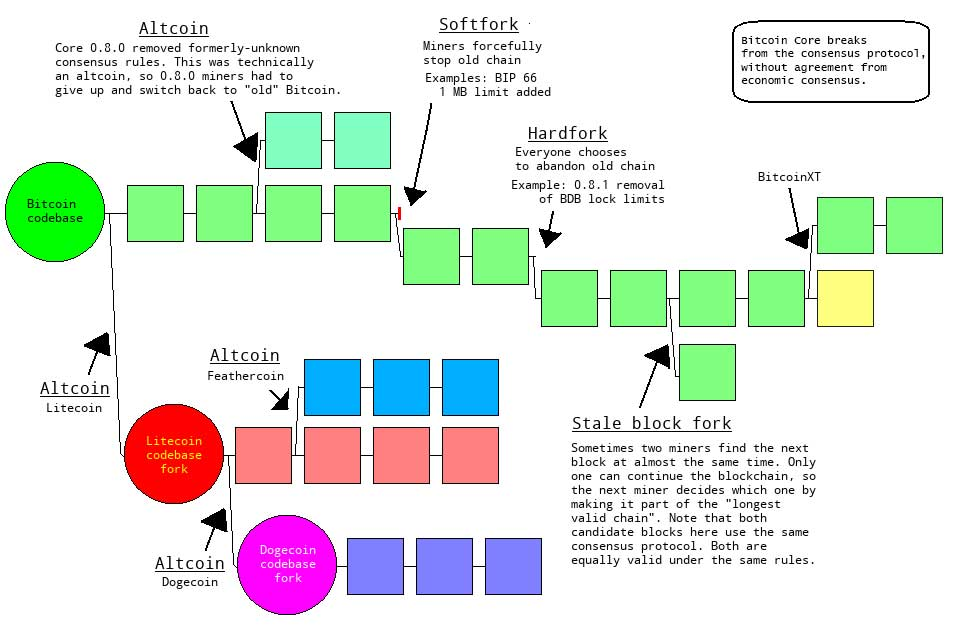
\includegraphics[width=1.0\linewidth]{images/altcoinsoftforksetc}
	\caption{Classificazione delle blockchain derivanti dalla codebase di Bitcoin.}
	\label{fig:altcoinsoftforksetc}
	\footnote{Fonte medium.com}
\end{figure}





\subsection{Litecoin}
Litecoin è una criptovaluta peer to peer che dal punto di vista tecnico condivide gran parte dell’implementazione di Bitcoin. Non è considerabile una fork di Bitcoin in senso stretto poiché non c’è stata la duplicazione della moneta, bensì una source code fork: è stato effettuato il fork del codice sorgente e del client open source Bitcoin Core e sono state effettuate delle modifiche sostanziali che si sono riflesse nella blockchain e le due valute non hanno uno storico comune. 
Nasce nel 2011 ad opera dell’ex ingegnere MIT Charlie Lee, con l’intento dichiarato di diventare rispetto a Bitcoin “ciò che l’argento è rispetto all’oro”; già da questa frase si può comprendere come Litecoin sia una valuta che si presta a micropagamenti e operazioni più rapide rispetto a Bitcoin. Lee sostiene di non aver concepito Litecoin come sostituto di Bitcoin, bensì come complemento per risolvere alcune criticità da lui rilevate.

Pur condividendone per la maggior parte struttura e protocollo presenta alcune differenze fondamentali:

Velocità: nel network Litecoin un blocco viene aggiunto alla Blockchain circa ogni 2.5 minuti contro i 10 di Bitcoin quadruplicando la velocità di creazione dei blocchi. Questo implica la possibilità di confermare le transazioni molto più rapidamente e a costi minori, nonché una minor congestione di rete e una riduzione del pericolo di attacchi double-spending a causa della finestra temporale utile ridotta.
La proof of work utilizza l’algoritmo Scrypt: per ridurre il pericolo di centralizzazione del calcolo nei nodi che possono permettersi hashing powers enormi tramite hardware pre-esistente specializzato per il mining.
Scrypt implementa alcune funzioni che fanno un largo uso di memoria per ridurre drasticamente l’efficienza dei circuiti logici tipici degli ASIC, privi di cache e ottimizzati per il mining intensivo. Trattandosi di un problema memory-hard sono privilegiate grandi quantità di RAM veloce. 
Questa scelta è stata fatta per evitare l’aumento esponenziale della difficoltà di mining in tempi brevi in un mercato in cui cominciavano già a prendere piede i suddetti dispositivi: Litecoin è nato oltre due anni dopo e la centralizzazione sarebbe stata un pericolo concreto.
84 milioni di unità monetarie, il quadruplo rispetto a Bitcoin.

I meccanismi di regolazione della difficoltà e di halving sono analoghi a Bitcoin ma i numeri cambiano: la difficoltà viene ricalcolata ogni 3.5 giorni -4 volte più velocemente- e l’halving è fissato ogni 840.000 blocchi -il quadruplo- in linea con la velocità e il numero di unità monetarie di Litecoin.

\subsubsection{Qualche dato su Litecoin}
Ad agosto 2018 risultano già minati e circolanti 57.000.000 Litecoin su un totale di 84.000.000 e il valore di un LTC fluttua intorno ai 60 euro.

\begin{figure}[h!]
	\centering
	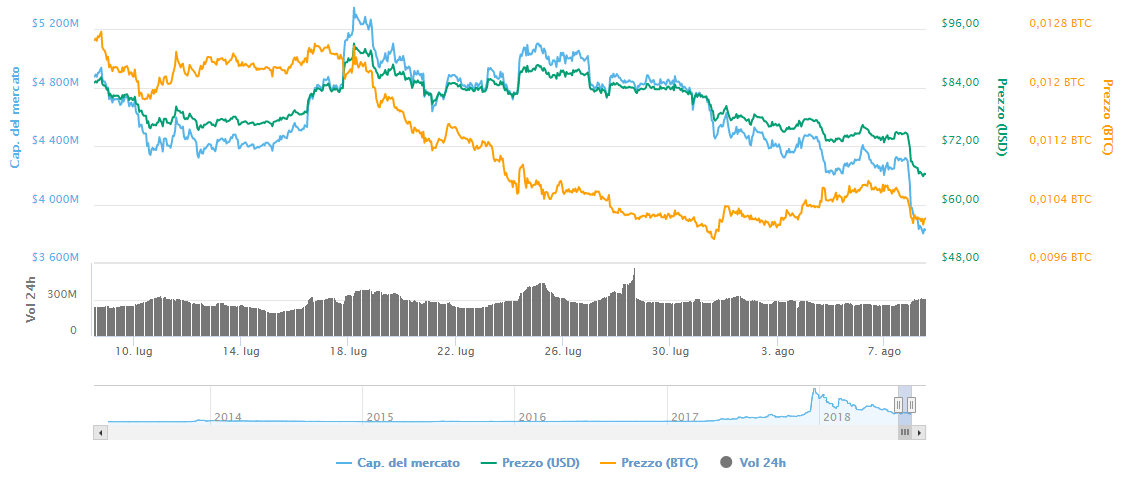
\includegraphics[width=1.0\linewidth]{images/LitecoinCoinMarketCap}
	\caption{Confronto tra gli andamenti di mercato di Bitcoin e Litecoin}
	\label{fig:litecoincoinmarketcap}
	\footnote{Fonte Coinmarketcap.com}
\end{figure}


Questo grafico illustra l’andamento sul mercato di Litecoin ed evidenzia come questo segua tendenzialmente l’andamento di Bitcoin.
Correntemente la difficoltà è prossima al $10^{7}$   \cite{bitcoinwisdom}, la ricompensa per un nuovo blocco ammonta a 25 LTC e il dimezzamento è previsto per il 6 agosto 2019.
La blockchain Litecoin contiene attualmente \~{}1.480.000 blocchi.

